\documentclass[twocolumn]{article}

\usepackage{blindtext} % Package to generate dummy text throughout this template 
\usepackage{flafter} 
\usepackage{graphicx}
\usepackage[sc]{mathpazo} % Use the Palatino font
\usepackage[T1]{fontenc} % Use 8-bit encoding that has 256 glyphs
\linespread{1.05} % Line spacing - Palatino needs more space between lines
\usepackage{microtype} % Slightly tweak font spacing for aesthetics
\usepackage{color}
\usepackage{listings}    
\usepackage{courier}

%%% Define Custom IDE Colors %%%
\definecolor{arduinoGreen}    {rgb} {0.17, 0.43, 0.01}
\definecolor{arduinoGrey}     {rgb} {0.47, 0.47, 0.33}
\definecolor{arduinoOrange}   {rgb} {0.8 , 0.4 , 0   }
\definecolor{arduinoBlue}     {rgb} {0.01, 0.61, 0.98}
\definecolor{arduinoDarkBlue} {rgb} {0.0 , 0.2 , 0.5 }

%%% Define Arduino Language %%%
\lstdefinelanguage{Arduino}{
  language=C++, % begin with default C++ settings 
%
%
  %%% Keyword Color Group 1 %%%  (called KEYWORD3 by arduino)
  keywordstyle=\color{arduinoGreen},   
  deletekeywords={  % remove all arduino keywords that might be in c++
                break, case, override, final, continue, default, do, else, for, 
                if, return, goto, switch, throw, try, while, setup, loop, export, 
                not, or, and, xor, include, define, elif, else, error, if, ifdef, 
                ifndef, pragma, warning,
                HIGH, LOW, INPUT, INPUT_PULLUP, OUTPUT, DEC, BIN, HEX, OCT, PI, 
                HALF_PI, TWO_PI, LSBFIRST, MSBFIRST, CHANGE, FALLING, RISING, 
                DEFAULT, EXTERNAL, INTERNAL, INTERNAL1V1, INTERNAL2V56, LED_BUILTIN, 
                LED_BUILTIN_RX, LED_BUILTIN_TX, DIGITAL_MESSAGE, FIRMATA_STRING, 
                ANALOG_MESSAGE, REPORT_DIGITAL, REPORT_ANALOG, SET_PIN_MODE, 
                SYSTEM_RESET, SYSEX_START, auto, int8_t, int16_t, int32_t, int64_t, 
                uint8_t, uint16_t, uint32_t, uint64_t, char16_t, char32_t, operator, 
                enum, delete, bool, boolean, byte, char, const, false, float, double, 
                null, NULL, int, long, new, private, protected, public, short, 
                signed, static, volatile, String, void, true, unsigned, word, array, 
                sizeof, dynamic_cast, typedef, const_cast, struct, static_cast, union, 
                friend, extern, class, reinterpret_cast, register, explicit, inline, 
                _Bool, complex, _Complex, _Imaginary, atomic_bool, atomic_char, 
                atomic_schar, atomic_uchar, atomic_short, atomic_ushort, atomic_int, 
                atomic_uint, atomic_long, atomic_ulong, atomic_llong, atomic_ullong, 
                virtual, PROGMEM,
                Serial, Serial1, Serial2, Serial3, SerialUSB, Keyboard, Mouse,
                abs, acos, asin, atan, atan2, ceil, constrain, cos, degrees, exp, 
                floor, log, map, max, min, radians, random, randomSeed, round, sin, 
                sq, sqrt, tan, pow, bitRead, bitWrite, bitSet, bitClear, bit, 
                highByte, lowByte, analogReference, analogRead, 
                analogReadResolution, analogWrite, analogWriteResolution, 
                attachInterrupt, detachInterrupt, digitalPinToInterrupt, delay, 
                delayMicroseconds, digitalWrite, digitalRead, interrupts, millis, 
                micros, noInterrupts, noTone, pinMode, pulseIn, pulseInLong, shiftIn, 
                shiftOut, tone, yield, Stream, begin, end, peek, read, print, 
                println, available, availableForWrite, flush, setTimeout, find, 
                findUntil, parseInt, parseFloat, readBytes, readBytesUntil, readString, 
                readStringUntil, trim, toUpperCase, toLowerCase, charAt, compareTo, 
                concat, endsWith, startsWith, equals, equalsIgnoreCase, getBytes, 
                indexOf, lastIndexOf, length, replace, setCharAt, substring, 
                toCharArray, toInt, press, release, releaseAll, accept, click, move, 
                isPressed, isAlphaNumeric, isAlpha, isAscii, isWhitespace, isControl, 
                isDigit, isGraph, isLowerCase, isPrintable, isPunct, isSpace, 
                isUpperCase, isHexadecimalDigit, 
                }, 
  morekeywords={   % add arduino structures to group 1
                break, case, override, final, continue, default, do, else, for, 
                if, return, goto, switch, throw, try, while, setup, loop, export, 
                not, or, and, xor, include, define, elif, else, error, if, ifdef, 
                ifndef, pragma, warning,
                }, 
% 
%
  %%% Keyword Color Group 2 %%%  (called LITERAL1 by arduino)
  keywordstyle=[2]\color{arduinoBlue},   
  keywords=[2]{   % add variables and dataTypes as 2nd group  
                HIGH, LOW, INPUT, INPUT_PULLUP, OUTPUT, DEC, BIN, HEX, OCT, PI, 
                HALF_PI, TWO_PI, LSBFIRST, MSBFIRST, CHANGE, FALLING, RISING, 
                DEFAULT, EXTERNAL, INTERNAL, INTERNAL1V1, INTERNAL2V56, LED_BUILTIN, 
                LED_BUILTIN_RX, LED_BUILTIN_TX, DIGITAL_MESSAGE, FIRMATA_STRING, 
                ANALOG_MESSAGE, REPORT_DIGITAL, REPORT_ANALOG, SET_PIN_MODE, 
                SYSTEM_RESET, SYSEX_START, auto, int8_t, int16_t, int32_t, int64_t, 
                uint8_t, uint16_t, uint32_t, uint64_t, char16_t, char32_t, operator, 
                enum, delete, bool, boolean, byte, char, const, false, float, double, 
                null, NULL, int, long, new, private, protected, public, short, 
                signed, static, volatile, String, void, true, unsigned, word, array, 
                sizeof, dynamic_cast, typedef, const_cast, struct, static_cast, union, 
                friend, extern, class, reinterpret_cast, register, explicit, inline, 
                _Bool, complex, _Complex, _Imaginary, atomic_bool, atomic_char, 
                atomic_schar, atomic_uchar, atomic_short, atomic_ushort, atomic_int, 
                atomic_uint, atomic_long, atomic_ulong, atomic_llong, atomic_ullong, 
                virtual, PROGMEM,
                },  
% 
%
  %%% Keyword Color Group 3 %%%  (called KEYWORD1 by arduino)
  keywordstyle=[3]\bfseries\color{arduinoOrange},
  keywords=[3]{  % add built-in functions as a 3rd group
                Serial, Serial1, Serial2, Serial3, SerialUSB, Keyboard, Mouse,
                },      
%
%
  %%% Keyword Color Group 4 %%%  (called KEYWORD2 by arduino)
  keywordstyle=[4]\color{arduinoOrange},
  keywords=[4]{  % add more built-in functions as a 4th group
                abs, acos, asin, atan, atan2, ceil, constrain, cos, degrees, exp, 
                floor, log, map, max, min, radians, random, randomSeed, round, sin, 
                sq, sqrt, tan, pow, bitRead, bitWrite, bitSet, bitClear, bit, 
                highByte, lowByte, analogReference, analogRead, 
                analogReadResolution, analogWrite, analogWriteResolution, 
                attachInterrupt, detachInterrupt, digitalPinToInterrupt, delay, 
                delayMicroseconds, digitalWrite, digitalRead, interrupts, millis, 
                micros, noInterrupts, noTone, pinMode, pulseIn, pulseInLong, shiftIn, 
                shiftOut, tone, yield, Stream, begin, end, peek, read, print, 
                println, available, availableForWrite, flush, setTimeout, find, 
                findUntil, parseInt, parseFloat, readBytes, readBytesUntil, readString, 
                readStringUntil, trim, toUpperCase, toLowerCase, charAt, compareTo, 
                concat, endsWith, startsWith, equals, equalsIgnoreCase, getBytes, 
                indexOf, lastIndexOf, length, replace, setCharAt, substring, 
                toCharArray, toInt, press, release, releaseAll, accept, click, move, 
                isPressed, isAlphaNumeric, isAlpha, isAscii, isWhitespace, isControl, 
                isDigit, isGraph, isLowerCase, isPrintable, isPunct, isSpace, 
                isUpperCase, isHexadecimalDigit, 
                },      
%
%
  %%% Set Other Colors %%%
  stringstyle=\color{arduinoDarkBlue},    
  commentstyle=\color{arduinoGrey},    
%          
%   
  %%%% Line Numbering %%%%
   numbers=left,                    
  numbersep=5pt,                   
  numberstyle=\color{arduinoGrey},    
  %stepnumber=2,                      % show every 2 line numbers
%
%
  %%%% Code Box Style %%%%
  breaklines=true,                    % wordwrapping
  tabsize=2,         
  basicstyle=\ttfamily  
}


\usepackage[english]{babel} % Language hyphenation and typographical rules

\usepackage[hmarginratio=1:1,top=32mm,columnsep=20pt]{geometry} % Document margins
\usepackage[hang, small,labelfont=bf,up,textfont=it,up]{caption} % Custom captions under/above floats in tables or figures
\usepackage{booktabs} % Horizontal rules in tables

\usepackage{lettrine} % The lettrine is the first enlarged letter at the beginning of the text

\usepackage{enumitem} % Customized lists
\setlist[itemize]{noitemsep} % Make itemize lists more compact

\usepackage{abstract} % Allows abstract customization
\renewcommand{\abstractnamefont}{\normalfont\bfseries} % Set the "Abstract" text to bold
\renewcommand{\abstracttextfont}{\normalfont\small\itshape} % Set the abstract itself to small italic text

\usepackage{titlesec} % Allows customization of titles
\renewcommand\thesection{\Roman{section}} % Roman numerals for the sections
\renewcommand\thesubsection{\roman{subsection}} % roman numerals for subsections
\titleformat{\section}[block]{\large\scshape\centering}{\thesection.}{1em}{} % Change the look of the section titles
\titleformat{\subsection}[block]{\large}{\thesubsection.}{1em}{} % Change the look of the section titles

\usepackage{fancyhdr} % Headers and footers
\pagestyle{fancy} % All pages have headers and footers
\fancyhead{} % Blank out the default header
\fancyfoot{} % Blank out the default footer
\fancyhead[C]{Electromagnetic Railgun $\bullet$ 1 November 2017} % Custom header text
\fancyfoot[RO,LE]{\thepage} % Custom footer text

\usepackage{titling} % Customizing the title section

\usepackage{hyperref} % For hyperlinks in the PDF

\setlength{\droptitle}{-4\baselineskip} % Move the title up

\pretitle{\begin{center}\Huge\bfseries} % Article title formatting
\posttitle{\end{center}} % Article title closing formatting
\title{Electromagnetic Railgun} % Article title
\author{%
\textsc{Aravind Ganesh}\\[1ex] % Your name
%\normalsize IITH \\ % Your institution
\normalsize \href{mailto:ee16tech11026@iith.ac.in}{ee16tech11026@iith.ac.in}
 % Your email address
\and % Uncomment if 2 authors are required, duplicate these 4 lines if more
\textsc{\textbf{Siva Kumar}}\\
 Project advisor\\
\normalsize \href{mailto:ksiva@iith.ac.in}{ksiva@iith.ac.in} % Second author's email address
\and % Uncomment if 2 authors are required, duplicate these 4 lines if more
\textsc{Adithya Hosapate}\\[1ex] % Second author's name
%\normalsize IITH \\ % Second author's institution
\normalsize \href{mailto:ee16btech11040@iith.ac.in}{ee16btech11040@iith.ac.in} % Second author's email address
\and % Uncomment if 2 authors are required, duplicate these 4 lines if more
\textsc{Anand N Warrier}\\[1ex] % Second author's name
%\normalsize IITH \\ % Second author's institution
\normalsize \href{mailto:ee16btech11042@iith.ac.in}{ee16btech11042@iith.ac.in} % Second author's email address
\and
\textsc{Deep Diwani}\\[1ex] % Your name
%\normalsize IITH \\ % Your institution
\normalsize \href{mailto:ee16tech11006@iith.ac.in}{ee16tech11006@iith.ac.in}
}

\date{\today} % Leave empty to omit a date
\renewcommand{\maketitlehookd}{%

}

%----------------------------------------------------------------------------------------

\begin{document}

% Print the title
\twocolumn[
\maketitle

\begin{abstract}

In this project, we have designed a prototype of a railgun. As this project is only for educational purposes, we have limited ourselves to low power levels of around 100V and 10 Amperes. We hope this project serves as a proof of concept. This prototype can be further developed and deployed in a multitude of applications.  

\end{abstract}
]
%----------------------------------------------------------------------------------------
%	ARTICLE CONTENTS
%----------------------------------------------------------------------------------------


\section{Introduction}

	A railgun is a device that uses electromagnetic force to launch high velocity projectiles, by means of a sliding armature that is accelerated along a pair of conductive rails. Railguns rely on electromagnetic force to propel a projectile at very high velocities(more than $3 km/s$).


\section{Potential Applications}
\begin{itemize}

\item Railguns are being researched as weapons that would use neither explosives nor propellant.The absence of explosive propellants or warheads to store and handle conventional weaponry come as additional advantages.

\item In addition to military applications, NASA has proposed to use a railgun to launch wedge-shaped aircraft with scramjets to high-altitude at Mach 10, where they will then fire a small payload into orbit using conventional rocket propulsion.

\item Railguns can potentially be used to aid mining, as a substitute for dynamite for clearing tunnels. 

\end{itemize}


\section{Principle}

The magnetic force on a current carrying conductor can be modelled by the equation. 
	
\begin{figure}[htp]
	\caption{Working principle of railgun}
	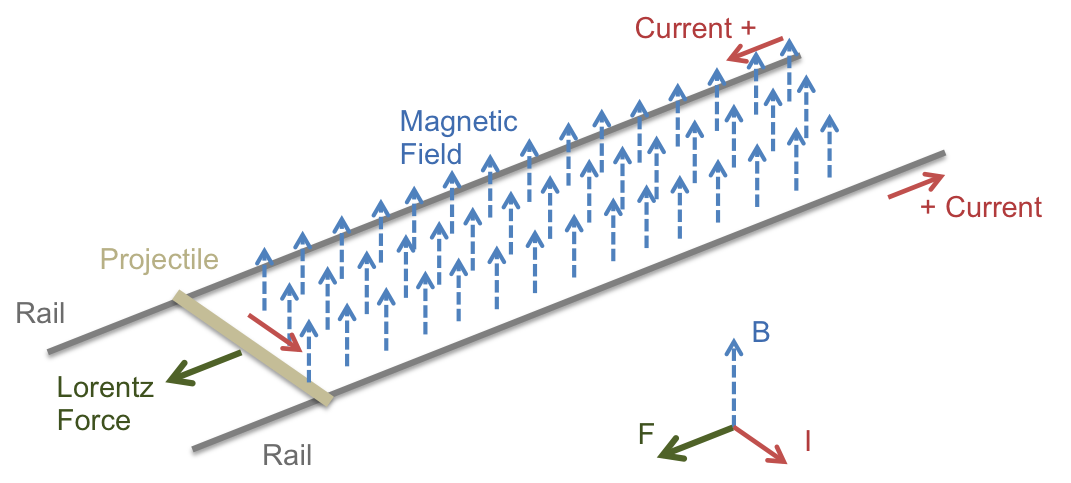
\includegraphics[width=\linewidth]{railgun_physics.png}
\end{figure}
	
\begin{equation}
\vec{F}=I_{r} \vec{l} \times \vec{B}
\end{equation}

Where $F$ is force, $B$ is magnetic field and $I_{r}$ is current passing through the rails.

As we are using permanent magnets to supply an external magnetic field, we restrict our power supply to DC only.
 
	We apply the magnetic field as seen in Figure 1 using strong permanent magnets. The magnetic field intensity of a magnet is given by $\vec{B}$
	

As the magnetic field is perpendicular to the current carrying projectile, $Eq(1)$ simplifies to
 \[|\vec{F}|=I_{r} l|\vec{B}|\]



 

\section{Approach}
We began by deciding the architecture of our gun.
After brainstorming many different setups, we settled on 

\begin{itemize}
\item A set of 2 parallel rails
\item A cylindrical graphite rod, which is conducting yet non-ferromagnetic.
\item Strong Permanent magnets to generate an external magnetic field
\item A capacitor bank in order to deliver high currents in a short amount of time to the rails.
\end{itemize}
\subsection*{\textbf{Current progress}} 
We began by designing the Capacitor bank charging circuit, using simulink (A MATLAB simulation software).

A detailed schematic of the circuit can be found below in Figure 1.
	\\
	
Figure 2 shows the voltage vs time plot of the charging capacitors.
	
\begin{figure}[htp]
	\caption{Circuit Diagram of simulated charging circuit}
	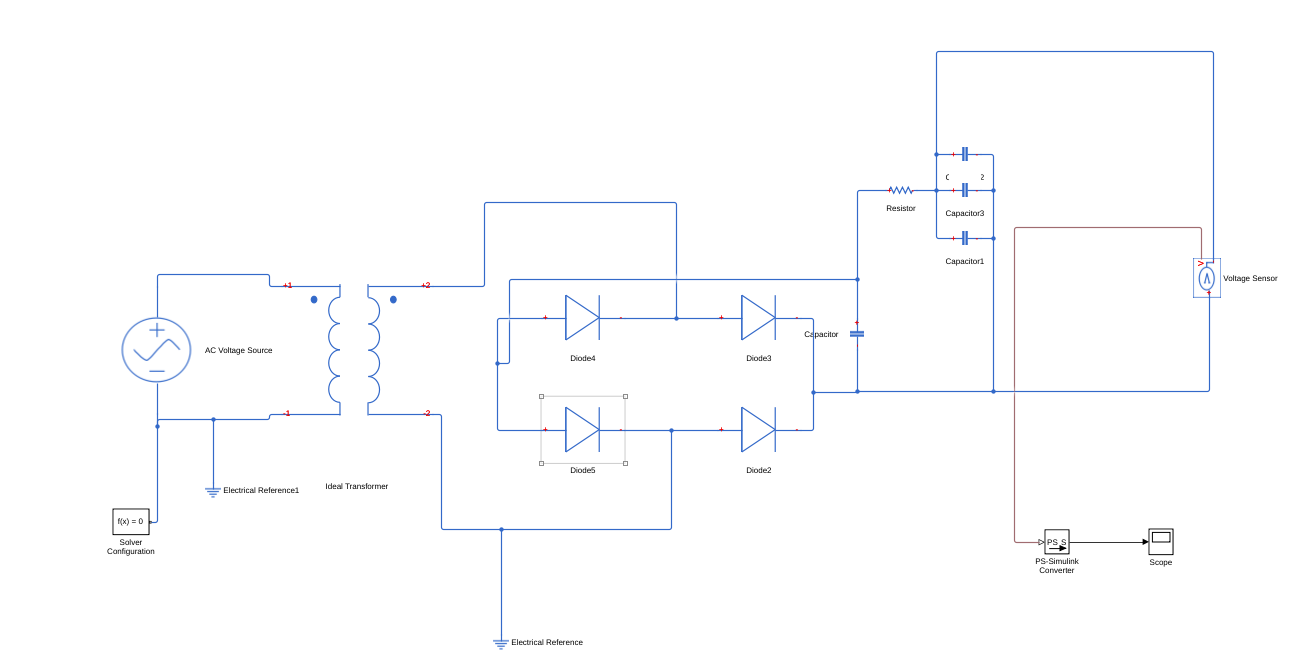
\includegraphics[width=\linewidth]{Circuit.png}
\end{figure}
	
	
\begin{figure}[h]
	\caption{Plot of voltage across capcitor bank vs time }
	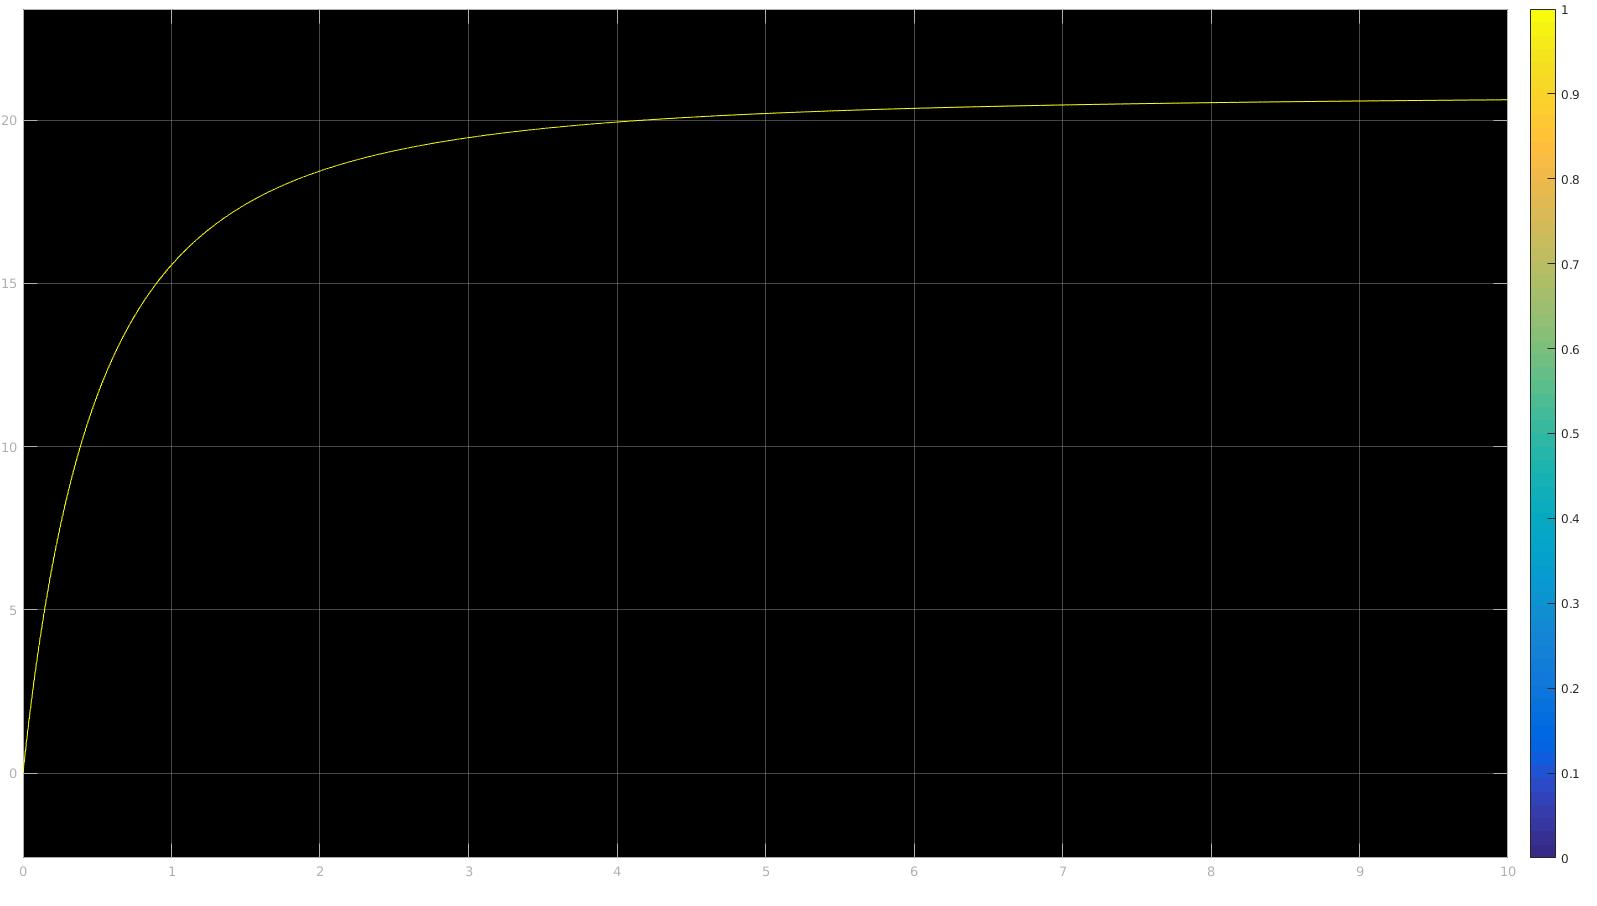
\includegraphics[width=\linewidth]{charging.jpg}
\end{figure}
		
	
We ran calculations using a matlab script and plotted the force on the projetile vs time along with the rail current vs time.(Figure 3)

\begin{figure}[h]
	\caption{Plots of rail current vs time and force vs time}
	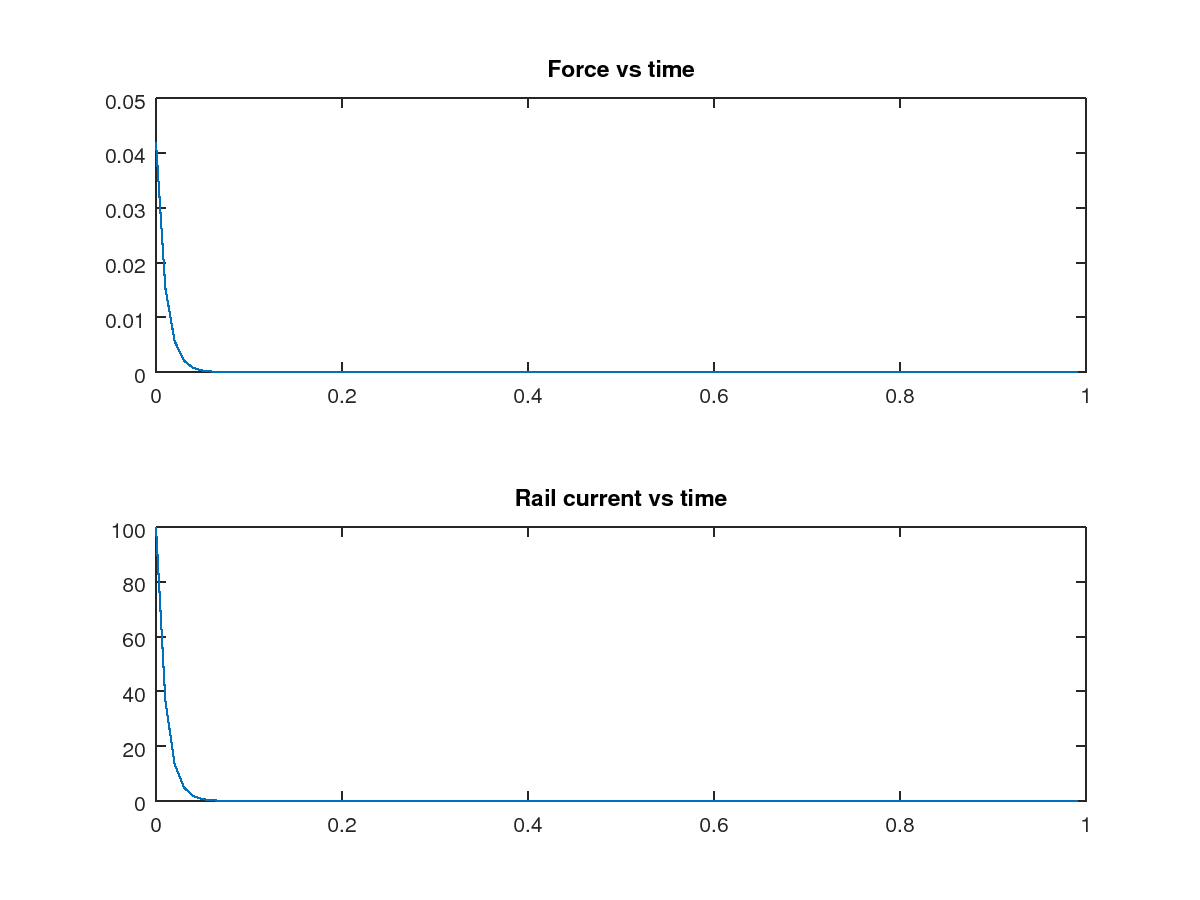
\includegraphics[width=\linewidth]{plots.png}
\end{figure}
		The script and all other code used in this project can be found in the project github repository.
\href{https://github.com/AravindGanesh/IDP-Sem3}{\textbf{https://github.com/AravindGanesh/IDP-Sem3}}



\section{Components}
\begin{itemize}
\item Capacitors - $2.2mF$  (as power source for the rails)
\item Variable Auto-Transformer 
\item Fullwave bridge Rectifier (uncontrolled)
\item Power MOSFET - IR740 (for switching)
\item Strong Neodymium Magnets
\item High power resistors
\item 
\item Steel scales as rails
\end{itemize}

\subsection*{Testing the Prototype}





\section{Bibliography} 
\begin{itemize}
\item https://www.allaboutcircuits.com.

\item electronics-course.com/ripple-counter.

\item https://www.eecs.tufts.edu/~dsculley/tutorial

\end{itemize}
%----------------------------------------------------------------------------------------

\end{document}
